%%%%%%%%%%%%%%%%%%%%%%%%%%%%%%%%%%%%%%%%%
% Jacobs Landscape Poster
% LaTeX Template
% Version 1.1 (14/06/14)
%
% Created by:
% Computational Physics and Biophysics Group, Jacobs University
% https://teamwork.jacobs-university.de:8443/confluence/display/CoPandBiG/LaTeX+Poster
% 
% Further modified by:
% Nathaniel Johnston (nathaniel@njohnston.ca)
%
% This template has been downloaded from:
% http://www.LaTeXTemplates.com
%
% License:
% CC BY-NC-SA 3.0 (http://creativecommons.org/licenses/by-nc-sa/3.0/)
%
%%%%%%%%%%%%%%%%%%%%%%%%%%%%%%%%%%%%%%%%%

%----------------------------------------------------------------------------------------
%	PACKAGES AND OTHER DOCUMENT CONFIGURATIONS
%----------------------------------------------------------------------------------------

\documentclass[final]{beamer}

\usepackage[scale=0.78,size=a1]{beamerposter} % Use the beamerposter package for laying out the poster

\usepackage{hyperref}

\usetheme{confposter} % Use the confposter theme supplied with this template

\setbeamercolor{block title}{fg=ngreen,bg=white} % Colors of the block titles
\setbeamercolor{block body}{fg=black,bg=white} % Colors of the body of blocks
\setbeamercolor{block alerted title}{fg=white,bg=dblue!70} % Colors of the highlighted block titles
\setbeamercolor{block alerted body}{fg=black,bg=dblue!10} % Colors of the body of highlighted blocks
% Many more colors are available for use in beamerthemeconfposter.sty

%-----------------------------------------------------------
% Define the column widths and overall poster size
% To set effective sepwid, onecolwid and twocolwid values, first choose how many columns you want and how much separation you want between columns
% In this template, the separation width chosen is 0.024 of the paper width and a 4-column layout
% onecolwid should therefore be (1-(# of columns+1)*sepwid)/# of columns e.g. (1-(4+1)*0.024)/4 = 0.22
% Set twocolwid to be (2*onecolwid)+sepwid = 0.464
% Set threecolwid to be (3*onecolwid)+2*sepwid = 0.708

\newlength{\sepwid}
\newlength{\onecolwid}
\newlength{\twocolwid}
\newlength{\threecolwid}
\setlength{\paperwidth}{36in} 
\setlength{\paperheight}{24in}
\setlength{\sepwid}{0.024\paperwidth} % Separation width (white space) between columns
\setlength{\onecolwid}{0.22\paperwidth} % Width of one column
\setlength{\twocolwid}{0.464\paperwidth} % Width of two columns
\setlength{\threecolwid}{0.708\paperwidth} % Width of three columns
\setlength{\topmargin}{-0.5in} % Reduce the top margin size
%-----------------------------------------------------------

\usepackage{graphicx}  % Required for including images
\usepackage{url}
\usepackage{caption}

\usepackage{booktabs} % Top and bottom rules for tables

%----------------------------------------------------------------------------------------
%	TITLE SECTION 
%----------------------------------------------------------------------------------------

\title{Unsupervised Learning of Religious Facial Features} % Poster title

\author{Christopher E. Mertin} % Author(s)

\institute{School of Computing, University of Utah} % Institution(s)

%----------------------------------------------------------------------------------------

\begin{document}

\addtobeamertemplate{block end}{}{\vspace*{2ex}} % White space under blocks
\addtobeamertemplate{block alerted end}{}{\vspace*{2ex}} % White space under highlighted (alert) blocks

\setlength{\belowcaptionskip}{2ex} % White space under figures
\setlength\belowdisplayshortskip{2ex} % White space under equations

\begin{frame}[t] % The whole poster is enclosed in one beamer frame

\begin{columns}[t] % The whole poster consists of three major columns, the second of which is split into two columns twice - the [t] option aligns each column's content to the top

\begin{column}{\sepwid}\end{column} % Empty spacer column

\begin{column}{\onecolwid} % The first column

%----------------------------------------------------------------------------------------
%	OBJECTIVES
%----------------------------------------------------------------------------------------

\begin{alertblock}{Abstract}
A paper published by N.O. Rule, {\em et. al}, explored the possibility of humans being able to discern if someone was part of a relgious group or not \cite{MormonID}, and was able to achieve 55\% accuracy. This paper explores the use of unsupervised learning techniques and eigenfaces to perform the same task, with clustering algorithms obtaining up to 59.3\% labeling accuracy on the clusters, and eigenfaces obtaining upwards of 80\% accuracy on unseen data. 
\end{alertblock}

%----------------------------------------------------------------------------------------
%	INTRODUCTION
%----------------------------------------------------------------------------------------

\begin{block}{Transforming the Data}

Need to transform the faces such that the corners of the eyes are in the same spot for each picture. This is done with the following equation.

\begin{align*}
  \begin{pmatrix}
    x^{\star} \\
    y^{\star}
\end{pmatrix} &= \begin{pmatrix}
\phi_{x}\cos(\theta) & \sin(\theta)\\
-\sin(\theta) & \phi_{y}\cos(\theta)
\end{pmatrix}  \begin{pmatrix}
    x \\
    y
\end{pmatrix} +   \begin{pmatrix}
    \psi_{x} \\
    \psi_{y}
\end{pmatrix}
\end{align*}

%------------------------------------------------

This transformation applied to a cropped image can be seen below.

\begin{figure}
\centering
\begin{minipage}{.5\textwidth}
  \centering
  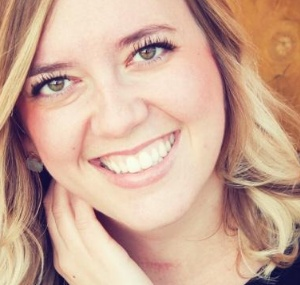
\includegraphics[width=.85\linewidth]{../data/Provo_Crop/Provo128-0_1.jpg}
  \captionof{figure}{Cropped Face}
  \label{fig:crop}
\end{minipage}%
\begin{minipage}{.5\textwidth}
  \centering
  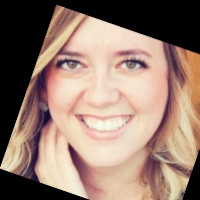
\includegraphics[width=.85\linewidth]{../data/Provo_Affine-color/Provo128-0_1.jpg}
  \captionof{figure}{Transformed Face}
  \label{fig:trans}
\end{minipage}
\end{figure}

We also need the ``average face'' of the two groups. This can be seen in the two figures below

\begin{figure}
\centering
\begin{minipage}{.5\textwidth}
  \centering
  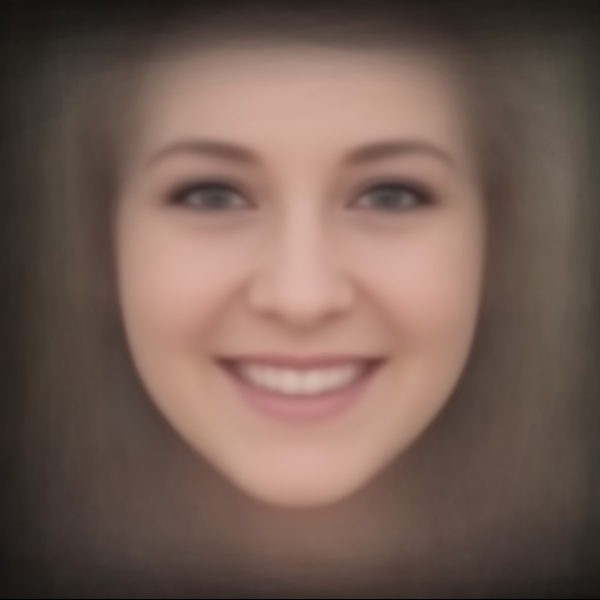
\includegraphics[width=.85\linewidth]{../data/Provo_avg.jpg}
  \captionof{figure}{Average Mormon Face}
  \label{fig:mo}
\end{minipage}%
\begin{minipage}{.5\textwidth}
  \centering
  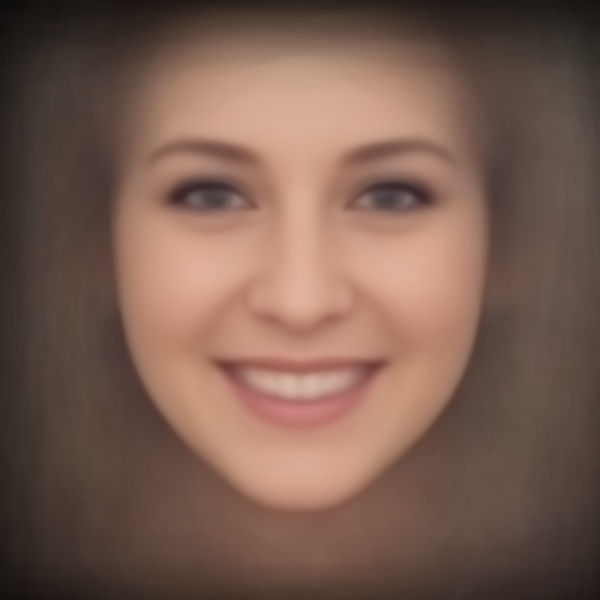
\includegraphics[width=.85\linewidth]{../data/Seattle_avg.jpg}
  \captionof{figure}{Average Non-Mormon Face}
  \label{fig:non_mo}
\end{minipage}
\end{figure}

\end{block}

%----------------------------------------------------------------------------------------

\end{column} % End of the first column

\begin{column}{\sepwid}\end{column} % Empty spacer column

\begin{column}{\onecolwid} % Begin a column which is two columns wide (column 2)

%----------------------------------------------------------------------------------------
%	MATERIALS
%----------------------------------------------------------------------------------------

\begin{block}{Eigenfaces}

To understand how much influence each singular value has, we can calculate the singular value variance by

\begin{align*}
  \frac{\sigma_{i}}{\sum_{i=1}^{N}\sigma_{i}}
\end{align*}

The variance shows that the majority of the data/images are represented within the first 50 singular values.

\begin{figure}
\centering
  \centering
  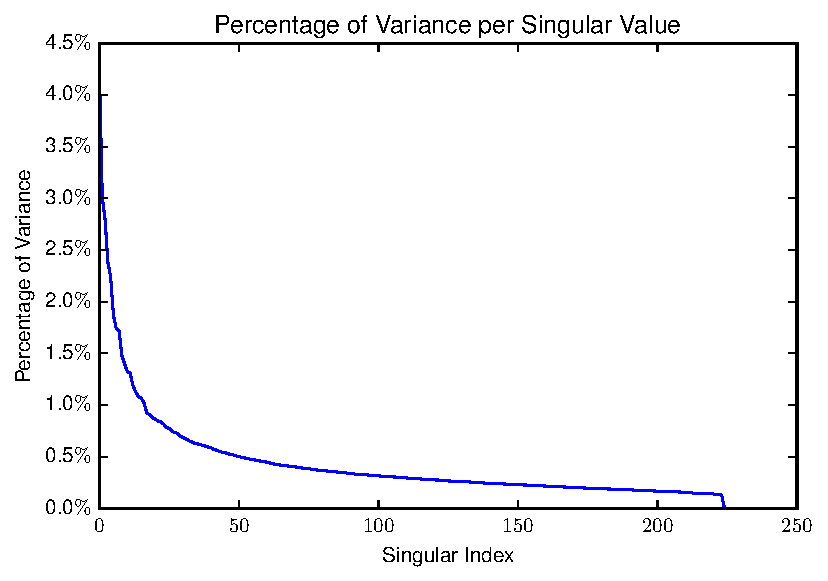
\includegraphics[width=.85\linewidth]{../data/Singularvalue_Variance.pdf}
  \captionof{figure}{Accuracy of Eigenfaces with various metrics}
  \label{fig:eig_acc}
\end{figure}

\begin{figure}
\centering
  \centering
  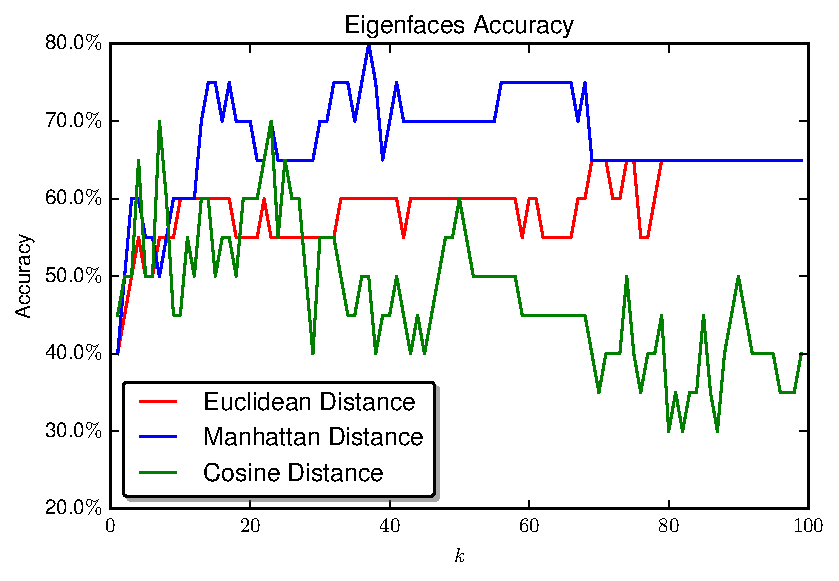
\includegraphics[width=.85\linewidth]{../data/Accuracy.pdf}
  \captionof{figure}{Accuracy of Eigenfaces with various metrics}
  \label{fig:eig_acc}
\end{figure}

\end{block}



\end{column} % End of column 2



%----------------------------------------------------------------------------------------
%	MATHEMATICAL SECTION
%----------------------------------------------------------------------------------------

\begin{column}{\sepwid}\end{column}

\begin{column}{\onecolwid}

\begin{block}{Agglomerative Clustering}

\begin{figure}
\centering
  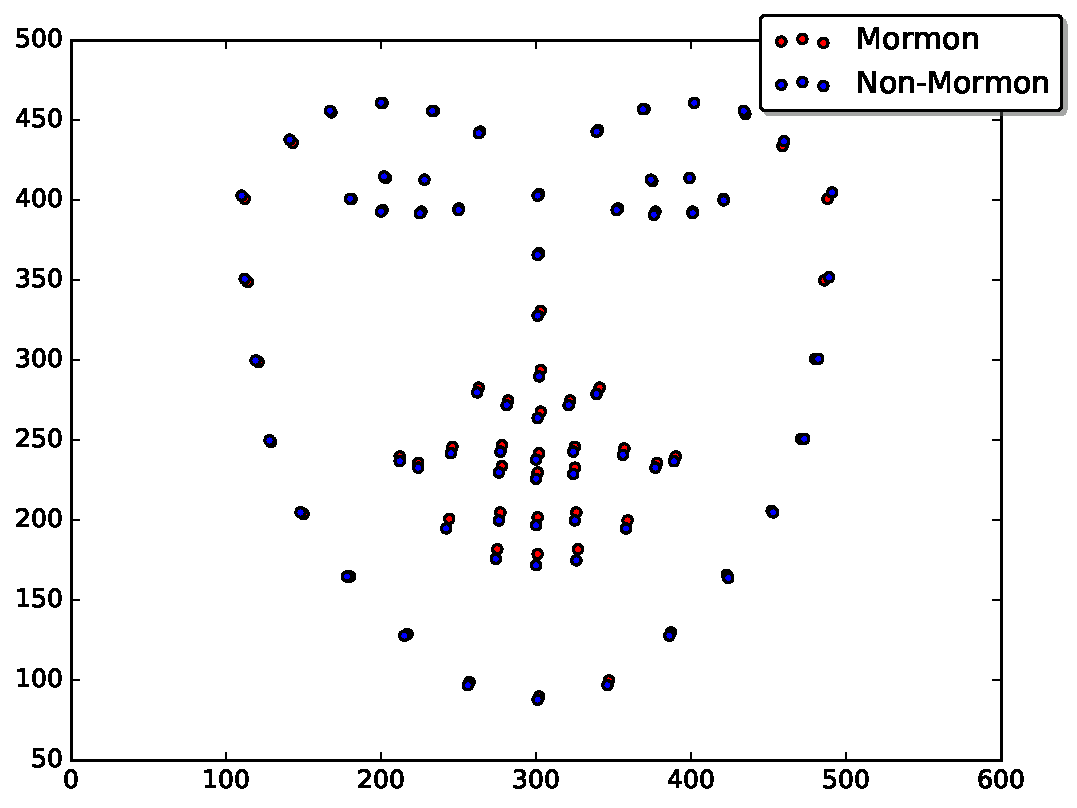
\includegraphics[width=.85\linewidth]{../data/average_sift.pdf}
  \captionof{figure}{SIFT Features of ``average faces''}
  \label{fig:sift_avg}
\end{figure}

\begin{figure}
\centering
  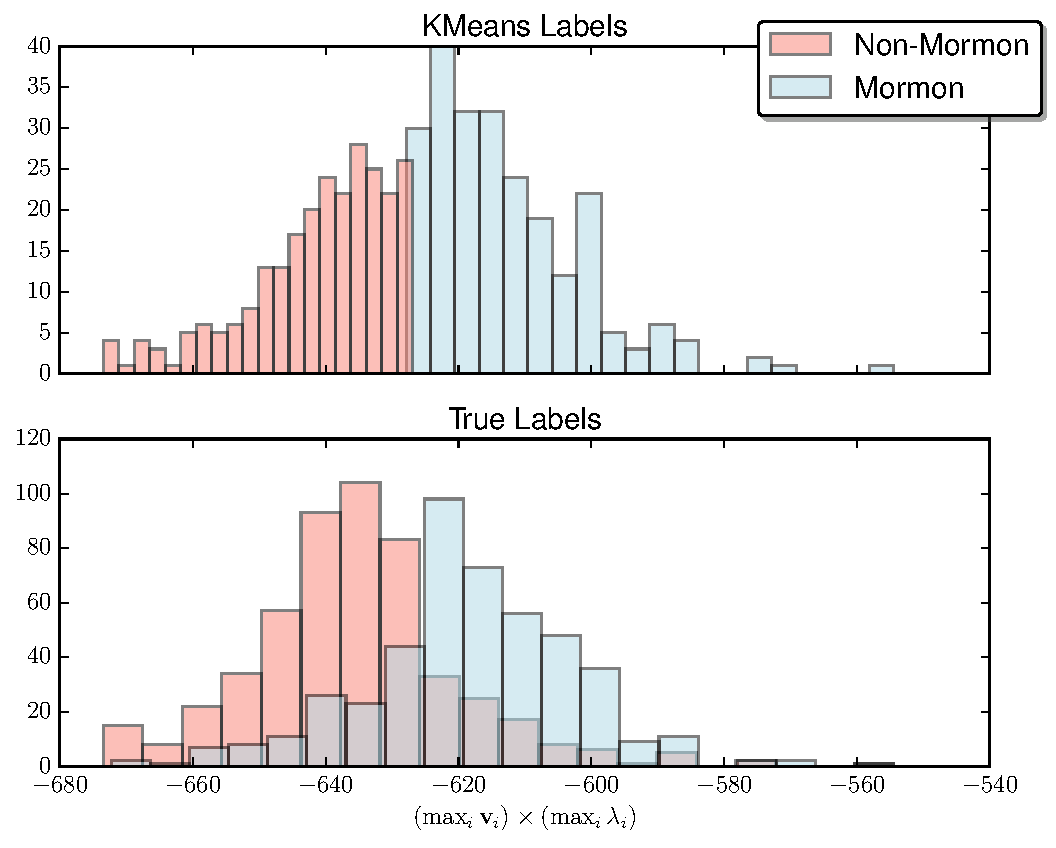
\includegraphics[width=.85\linewidth]{../data/eigennorm.pdf}
  \captionof{figure}{Labeling based on largest eigenvector and eigenvalue}
  \label{fig:eigennorm}
\end{figure}

\end{block}

%----------------------------------------------------------------------------------------


\end{column} % End of column 2.2


\begin{column}{\sepwid}\end{column} % Empty spacer column

\begin{column}{\onecolwid} % The third column

%----------------------------------------------------------------------------------------
%	CONCLUSION
%----------------------------------------------------------------------------------------

\begin{block}{Conclusion}

In conclusion, the unsupervised algorithms such as hierarchical clustering and KMeans did better than humans in \cite{MormonID}, with hierarchical clustering obtaining 58.4\% accuracy and KMeans 59.3\%. 

The Eigenfaces algorithm performed much better with various values of $k$ and the metric. The best metric was the Manhattan Distance which was able to achieve up to 80\% labeling accuracy for $k \sim 35$. On average, the manhattan distance performed much better than either of the aforementioned clustering algorithms.

All implementations performed better than humans in \cite{MormonID}.

\end{block}

%----------------------------------------------------------------------------------------
%	REFERENCES
%----------------------------------------------------------------------------------------

\begin{block}{References}

\nocite{*} % Insert publications even if they are not cited in the poster
\small{\bibliographystyle{unsrt}
\bibliography{bibliography}\vspace{0.75in}}

\end{block}

%----------------------------------------------------------------------------------------
%	ACKNOWLEDGEMENTS
%----------------------------------------------------------------------------------------

%----------------------------------------------------------------------------------------
%	CONTACT INFORMATION
%----------------------------------------------------------------------------------------

\setbeamercolor{block alerted title}{fg=black,bg=norange} % Change the alert block title colors
\setbeamercolor{block alerted body}{fg=black,bg=white} % Change the alert block body colors

\begin{alertblock}{Contact Information}

\begin{itemize}
\item Web: \href{http://cmertin.github.io}{\url{https://cmertin.github.io/}}
\item Email: \href{mailto:cmertin@cs.utah.edu}{\verb~cmertin@cs.utah.edu~}
\end{itemize}

\end{alertblock}


%----------------------------------------------------------------------------------------

\end{column} % End of the third column

\end{columns} % End of all the columns in the poster

\end{frame} % End of the enclosing frame

\end{document}
